%%%%%%%%%%%%%%%%%%%%%%%%%%%%%%%%%%%%%%%%%
% University/School Laboratory Report
% LaTeX Template
% Version 3.1 (25/3/14)
%
% This template has been downloaded from:
% http://www.LaTeXTemplates.com
%
% Original author:
% Linux and Unix Users Group at Virginia Tech Wiki 
% (https://vtluug.org/wiki/Example_LaTeX_chem_lab_report)
%
% License:
% CC BY-NC-SA 3.0 (http://creativecommons.org/licenses/by-nc-sa/3.0/)
%
%%%%%%%%%%%%%%%%%%%%%%%%%%%%%%%%%%%%%%%%%

%----------------------------------------------------------------------------------------
%	PACKAGES AND DOCUMENT CONFIGURATIONS
%----------------------------------------------------------------------------------------

\documentclass{article}

\usepackage{graphicx} % Required for the inclusion of images
\usepackage{natbib} % Required to change bibliography style to APA
\usepackage{amsmath} % Required for some math elements 
\usepackage{listings}
\usepackage{color}
\usepackage{fancyvrb}
\usepackage[margin=1in]{geometry}

\definecolor{dkgreen}{rgb}{0,0.6,0}
\definecolor{gray}{rgb}{0.5,0.5,0.5}
\definecolor{mauve}{rgb}{0.58,0,0.82}
\definecolor{black}{rgb}{0,0,0}

\lstset{frame=tb,
    language=R,
    aboveskip=3mm,
    belowskip=3mm,
    showstringspaces=false,
    columns=flexible,
    basicstyle={\small\ttfamily},
    numbers=none,
    numberstyle=\tiny\color{gray},
    keywordstyle=\color{blue},
    commentstyle=\color{dkgreen},
    stringstyle=\color{mauve},
    breaklines=true,
    breakatwhitespace=true,
    tabsize=3
}

\setlength\parindent{0pt} % Removes all indentation from paragraphs
% redefine \VerbatimInput
\RecustomVerbatimCommand{\VerbatimInput}{VerbatimInput}
{
    fontsize=\footnotesize,
    frame=lines,  % top and bottom rule only
    framesep=2em, % separation between frame and text
    rulecolor=\color{black},
    label=\fbox{\color{black}main.R},
    labelposition=topline,
    commentchar=*        % comment character
}

% Make numbering in the enumerate environment by letter rather than number
\renewcommand{\labelenumi}{\alph{enumi}.}

%----------------------------------------------------------------------------------------
%	DOCUMENT INFORMATION
%----------------------------------------------------------------------------------------

\title{Project 1 \\ STAT 355} % Title
\author{Sabbir \textsc{Ahmed}} % Author name
\date{\today} % Date for the report

\begin{document}

    \maketitle % Insert the title, author and date

    \section{Part 1}
        1000 random numbers were generated using a Bernoulli random variable with n = 20, p = 0.4
\begin{lstlisting}
    # initialize parameters for binomial distribution
    x <- 20
    N <- 1000
    p <- 0.4
    generatedData <- rbinom(N, x, p)
\end{lstlisting}

        \subsection{Distribution}
            Distribution of the data was plotted with a histogram using ggplot2 in Figure \ref{fig:hist}.
\begin{lstlisting}
    # plot a histogram
    ggplot() + aes(generatedData) + 
        geom_histogram(binwidth=1, color="black", fill="white") + labs(y="Count")
\end{lstlisting}

            \begin{figure}[h]
                \begin{center}
                    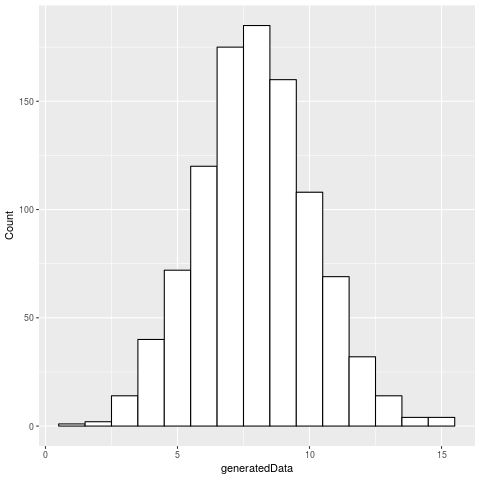
\includegraphics[width=0.6\textwidth]{figures/hist.png}
                    \caption{Histogram of the Generated Data} \label{fig:hist}
                \end{center}
            \end{figure}

        \subsection{Mean, Variance, and Standard Deviation}
            The mean, variance and standard deviation of the data were computed with the following snippet to generate Table 1:
\begin{lstlisting}
    # print out the mean, variance and standard deviation
    paste("Mean:", signif(mean(generatedData), digits=4),
        "| Variance:", signif(var(generatedData), digits=4),
        "| Standard Deviation:", signif(sqrt(var(generatedData)), digits=4))
\end{lstlisting}

        \renewcommand{\arraystretch}{1.5}
        \setlength{\tabcolsep}{18pt}
        \begin{table}[h!]
            \centering
            \begin{tabular}{|p{3cm}|p{3cm}|p{3cm}|}
                 \hline
                 \multicolumn{3}{|c|}{Table 1: Statistics} \\
                 \hline
                 Mean & Variance & Standard Deviation\\
                 \hline
                 7.953 & 4.832 & 2.198\\
                 \hline
            \end{tabular}
        \end{table}

        \subsection{Summary}
            Summary statistics were generated with the following snippet to generate Table 2:
\begin{lstlisting}
    # print out the summary statistics
    summary(generatedData)
\end{lstlisting}

        \begin{table}[h!]
            \centering
            \begin{tabular}{|p{1.5cm}|p{1.5cm}|p{1.5cm}|p{1.5cm}|p{1.5cm}|p{1.5cm}|}
                 \hline
                 \multicolumn{6}{|c|}{Table 2: Summary Statistics} \\
                 \hline
                   Minimum & 1st Quar. &  Median & Mean & 3rd Quar. & Maximum \\
                 \hline
                 1.000 & 7.000 & 8.000 & 7.953 & 9.000 & 15.000\\
                 \hline
            \end{tabular}
        \end{table}

        \subsection{Relative Frequencies}
            The frequencies and relative frequencies of the generate data were computed with the following snippet:
\begin{lstlisting}
    # frequencies
    ftable(generatedData)

    # relative frequencies
    ftable(generatedData)/N
\end{lstlisting}

            The relative frequencies were then plotted in a barplot as in Figure \ref{fig:relfreq}:
\begin{lstlisting}
    # generate barplot of the relative frequencies
    ggplot(data=relfreq, aes(x=generatedData, y=Freq)) + 
        geom_bar(color="black", fill="white", stat="identity") +
        labs(y="Relative Frequency")
\end{lstlisting}

            \begin{figure}[h]
                \begin{center}
                    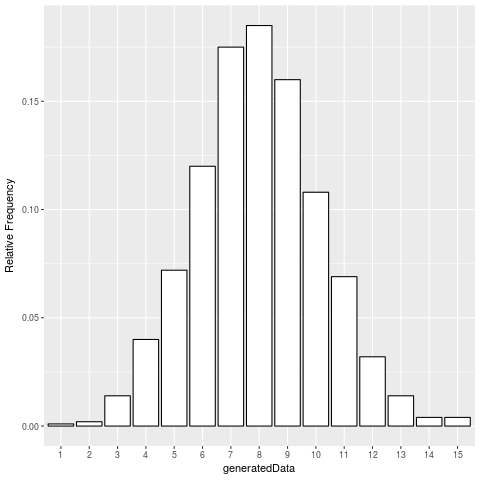
\includegraphics[width=0.6\textwidth]{figures/relfreq.png}
                    \caption{Relative Frequencies of the Generated Data} \label{fig:relfreq}
                \end{center}
            \end{figure}

        \subsection{Binomial Table}
            The cumulative probability $P(X=x)$ of the relative frequencies were computed with the following snippet to generate Figure \ref{fig:cumProb}:
\begin{lstlisting}
    # print out the cumulative probability to compare with the binomial 
    # distribution table
    cumProb <- 0  # initialize binomial cumulative probability

    # iterate through the entire dataframe
    for (i in 1:(nrow(relfreq))) {
        cumProb=cumProb+relfreq[i, "Freq"]
        print(
            paste0(
                "b(", relfreq[i, "generatedData"], ', ', x, ', ', p, ") -> ",
                cumProb
            )
        )
    }
\end{lstlisting}


            \begin{figure}[h]
                \begin{center}
                    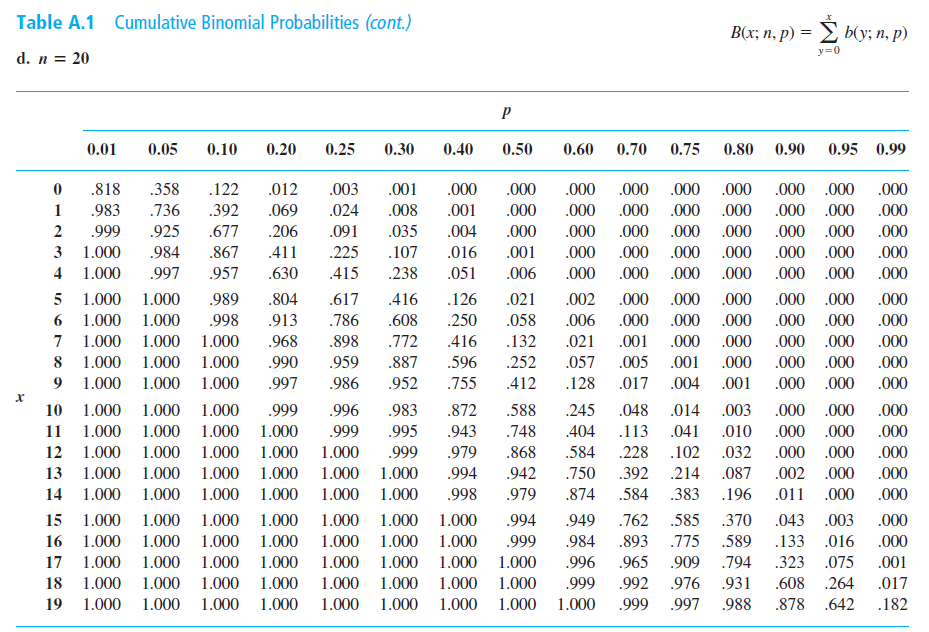
\includegraphics[width=0.6\textwidth]{figures/binom_table.png}
                    \caption{Cumulative Binomial Probability Table from the Textbook} \label{fig:binom_table}
                \end{center}
            \end{figure}


            \begin{figure}[h]
                \begin{center}
                    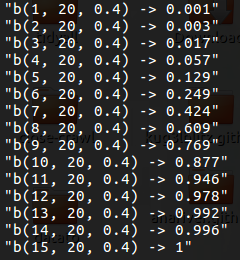
\includegraphics[width=0.4\textwidth]{figures/cumProb.png}
                    \caption{Cumulative Binomial Probability Generated} \label{fig:cumProb}
                \end{center}
            \end{figure}

    \section{Part 2}
    A very large batch of components has arrived at a distributor. The batch can be characterized as acceptable only if the proportion of defective components is at most 0.10. The distributor decides to randomly select 10 components and to accept the batch only if the number of defective components in the sample is at most 2.

        \subsection{Probability}
            The probabilities of accepting the lot were computed with the proportion of defective components as p = 0.01, 0.05, 0.10, 0.20, 0.25.

\begin{lstlisting}
    # initialize variables
    probs <- c(0.01, 0.05, 0.10, 0.20, 0.25)
    proportions <- rep(0, times=length(probs))

    # generate binomial probabilities with b(2, 10, p)
    for (i in 1:length(proportions)) {
        proportions[i] = signif(pbinom(2, size=10, prob=probs[i]), digits=4)
    }
    bnomDF <- data.frame(p=probs, px=proportions)
\end{lstlisting}


        \subsection{Characteristic Curve}
            The characteristic curve for the acceptance sampling plan was generated as Figure \ref{fig:charcurve1} with the following snippet:

\begin{lstlisting}
    # plot the characteristic curve
    ggplot(bnomDF, aes(x=p, y=px)) + geom_line() + geom_point(color="red") +
        labs(x="p", y="P(Acceptance)")
\end{lstlisting}

            \begin{figure}[h]
                \begin{center}
                    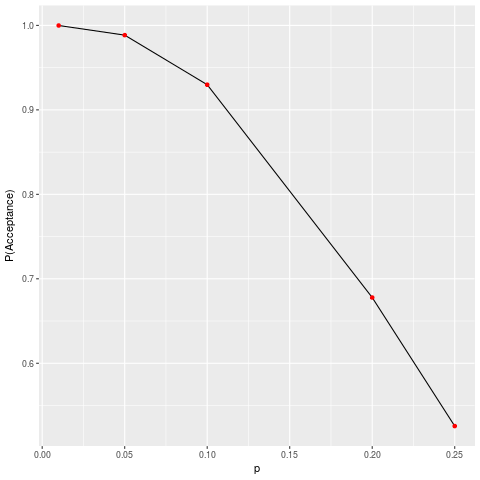
\includegraphics[width=0.6\textwidth]{figures/charcurve1.png}
                    \caption{Relative Frequencies of the Generated Data (Part A)} \label{fig:charcurve1}
                \end{center}
            \end{figure}


        \subsection{Probability with Different Maximum Acceptable Sample}
            The probabilities of accepting the lot were computed with the same proportions of defective components with the maximum sample changed to 1 and its characteristic curve was plotted as Figure \ref{fig:charcurve2}

\begin{lstlisting}
    # generate binomial probabilities with b(1, 10, p)
    for (i in 1:length(proportions)) {
        proportions[i] = signif(pbinom(1, size=10, prob=probs[i]), digits=4)
    }
    bnomDF <- data.frame(p=probs, px=proportions)
\end{lstlisting}

            \begin{figure}[h]
                \begin{center}
                    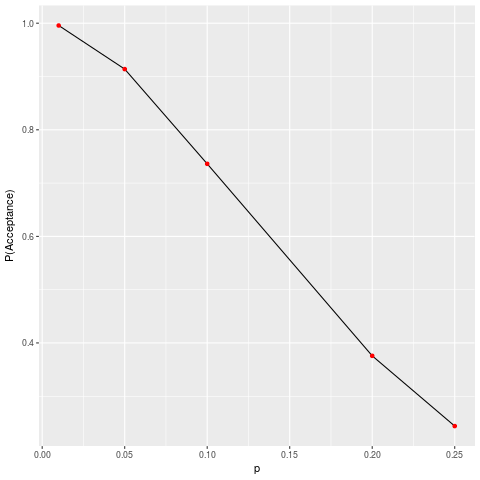
\includegraphics[width=0.6\textwidth]{figures/charcurve2.png}
                    \caption{Relative Frequencies of the Generated Data (Part C)} \label{fig:charcurve2}
                \end{center}
            \end{figure}

        \subsection{Probability with Different Sample Size}
            The probabilities of accepting the lot were computed with the same proportions of defective components with the sample size changed to 15 and its characteristic curve was plotted as Figure \ref{fig:charcurve3}

\begin{lstlisting}
    # generate binomial probabilities with b(2, 15, p)
    for (i in 1:length(proportions)) {
        proportions[i] = signif(pbinom(2, size=15, prob=probs[i]), digits=4)
    }
    bnomDF <- data.frame(p=probs, px=proportions)
\end{lstlisting}

            \begin{figure}[h]
                \begin{center}
                    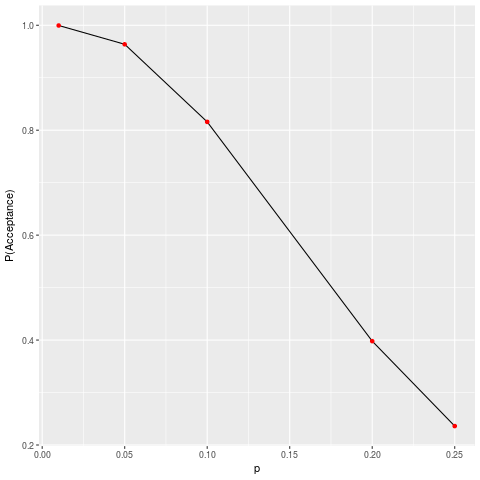
\includegraphics[width=0.6\textwidth]{figures/charcurve3.png}
                    \caption{Relative Frequencies of the Generated Data (Part D)} \label{fig:charcurve3}
                \end{center}
            \end{figure}

        \subsection{Outcomes}
            The second characteristic curve (Part C, Figure \ref{fig:charcurve2}) seems to be the most satisfactory because of its near linear relationship between the proportion and their probability.

    \clearpage
    \newpage
    \VerbatimInput{main.R}


\end{document}
